\chapter{Expériences}
\graphicspath{{04-Analyse/}}

Cette section présente les différentes expériences réalisées afin de mieux comprendre l'architecture CxSOM.
En utilisant les indicateurs et tracés présentés dans le chapitre précédent, nous détaillons dans cette partie les résltats obtenus et les pistes d'interprétation.

Les jeux de données présentés aux cartes de l'architecture sont des nuages de points en deux ou trois dimensions, tirés selon une distribution.
Les données d'entrée à l'architecture de carte seront notées $X$,$Y$,$Z$, sauf mention contraire. Ces trois valeurs sont scalaires, sont les coordonnées d'un point du nuage de point, et correspondent chacune à l'entrée d'une des cartes de l'architecture.

\section{Deux cartes}

Une architecture de deux cartes, connectées mutuellement, est l'exemple le plus simple d'architecture CxSOM. Son étude permet de dégager des comportements facilement représentables d'un point de vue graphique et ayant peu de liberté possible. 


\subsection{Entrées sur un cercle}

Prenons en entrée $(X,Y)$ situé sur n cercle de centre 0.5 et de rayon 0.5, tel que $X,Y \in [0,1]$. 
Les entrées de chacune des cartes sont donc dépendantes. Nous regarderons la distribution des valeurs selon les BMU de chaque carte.
\begin{figure}
\begin{minipage}{0.33\textwidth}
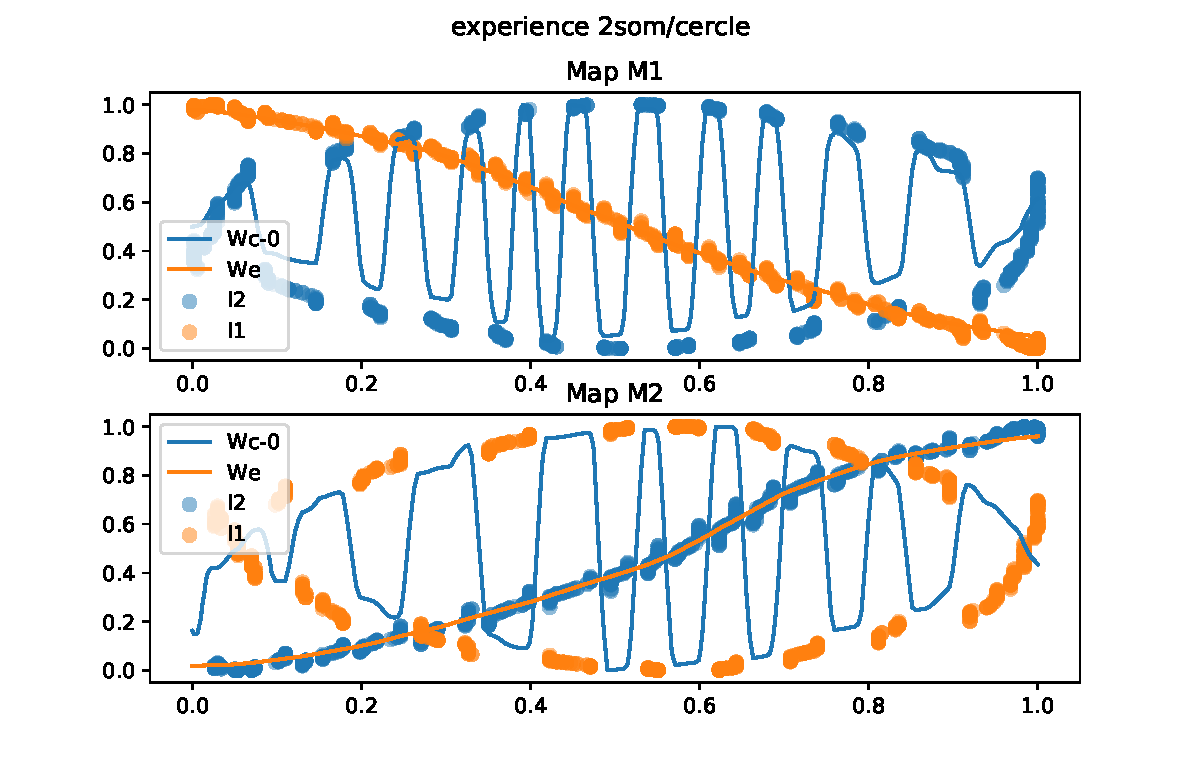
\includegraphics[width=\textwidth]{2som_cercle_w.pdf}
\end{minipage}
\begin{minipage}{0.33\textwidth}
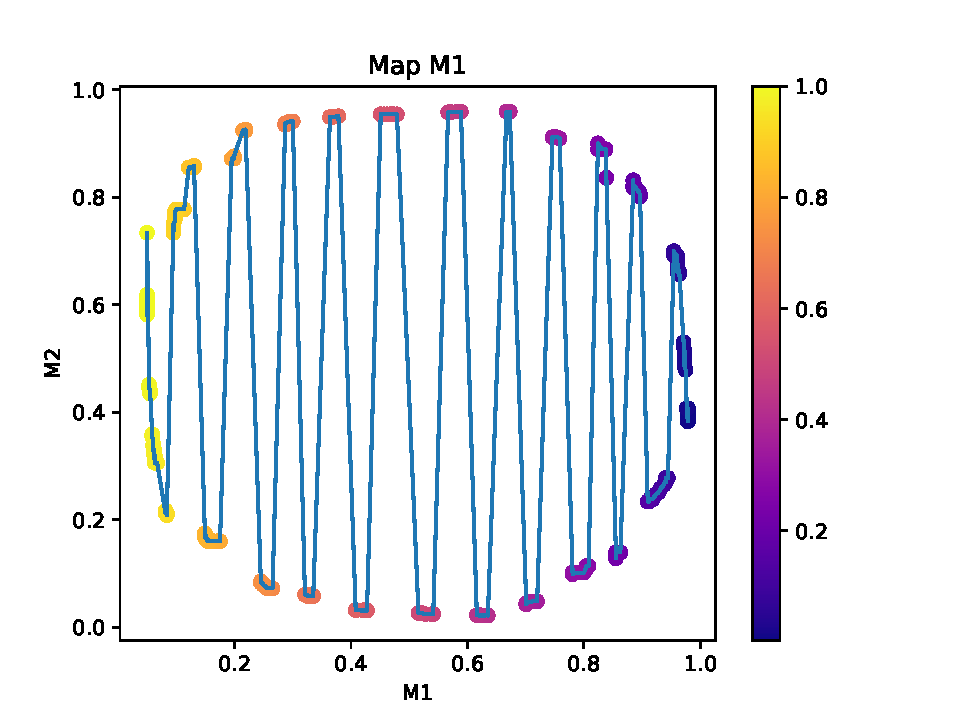
\includegraphics[width=\textwidth]{2som_cercle_d.pdf}
\end{minipage}
\begin{minipage}{0.33\textwidth}
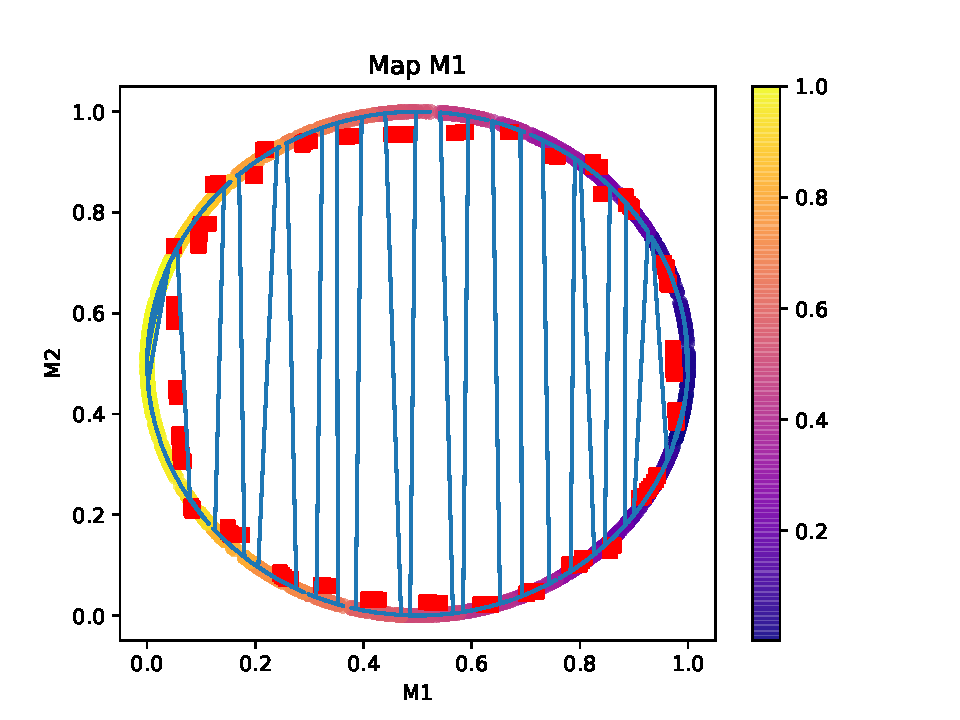
\includegraphics[width=\textwidth]{2som_cercle_din.pdf}
\end{minipage}
\label{fig:2som_square}
\caption{Tracé des poids de M1 et M2, dépliement des poids de M1 dans l'espace 2D et dépliement des entrées}
\end{figure}

\subsection{Entrées dans un carré}

\subsubsection{Expérience}
Prenons en entrée $(X,Y) \in [0,1]^2$, tirés selon une distribution uniforme. Les entrées de chacune des cartes sont donc indépendantes. Nous regarderons la distribution des valeurs selon les BMU de chaque carte. Cette distribution de valeurs dépendra donc uniquement de l'architecture, étant données que les entrées n'ont aucun lien entre elles. Cela nous permet de visualiser quels comportements sont uniquement issus du modèle.
 
\subsubsection{Résultats}

\begin{figure}
\begin{minipage}{0.33\textwidth}
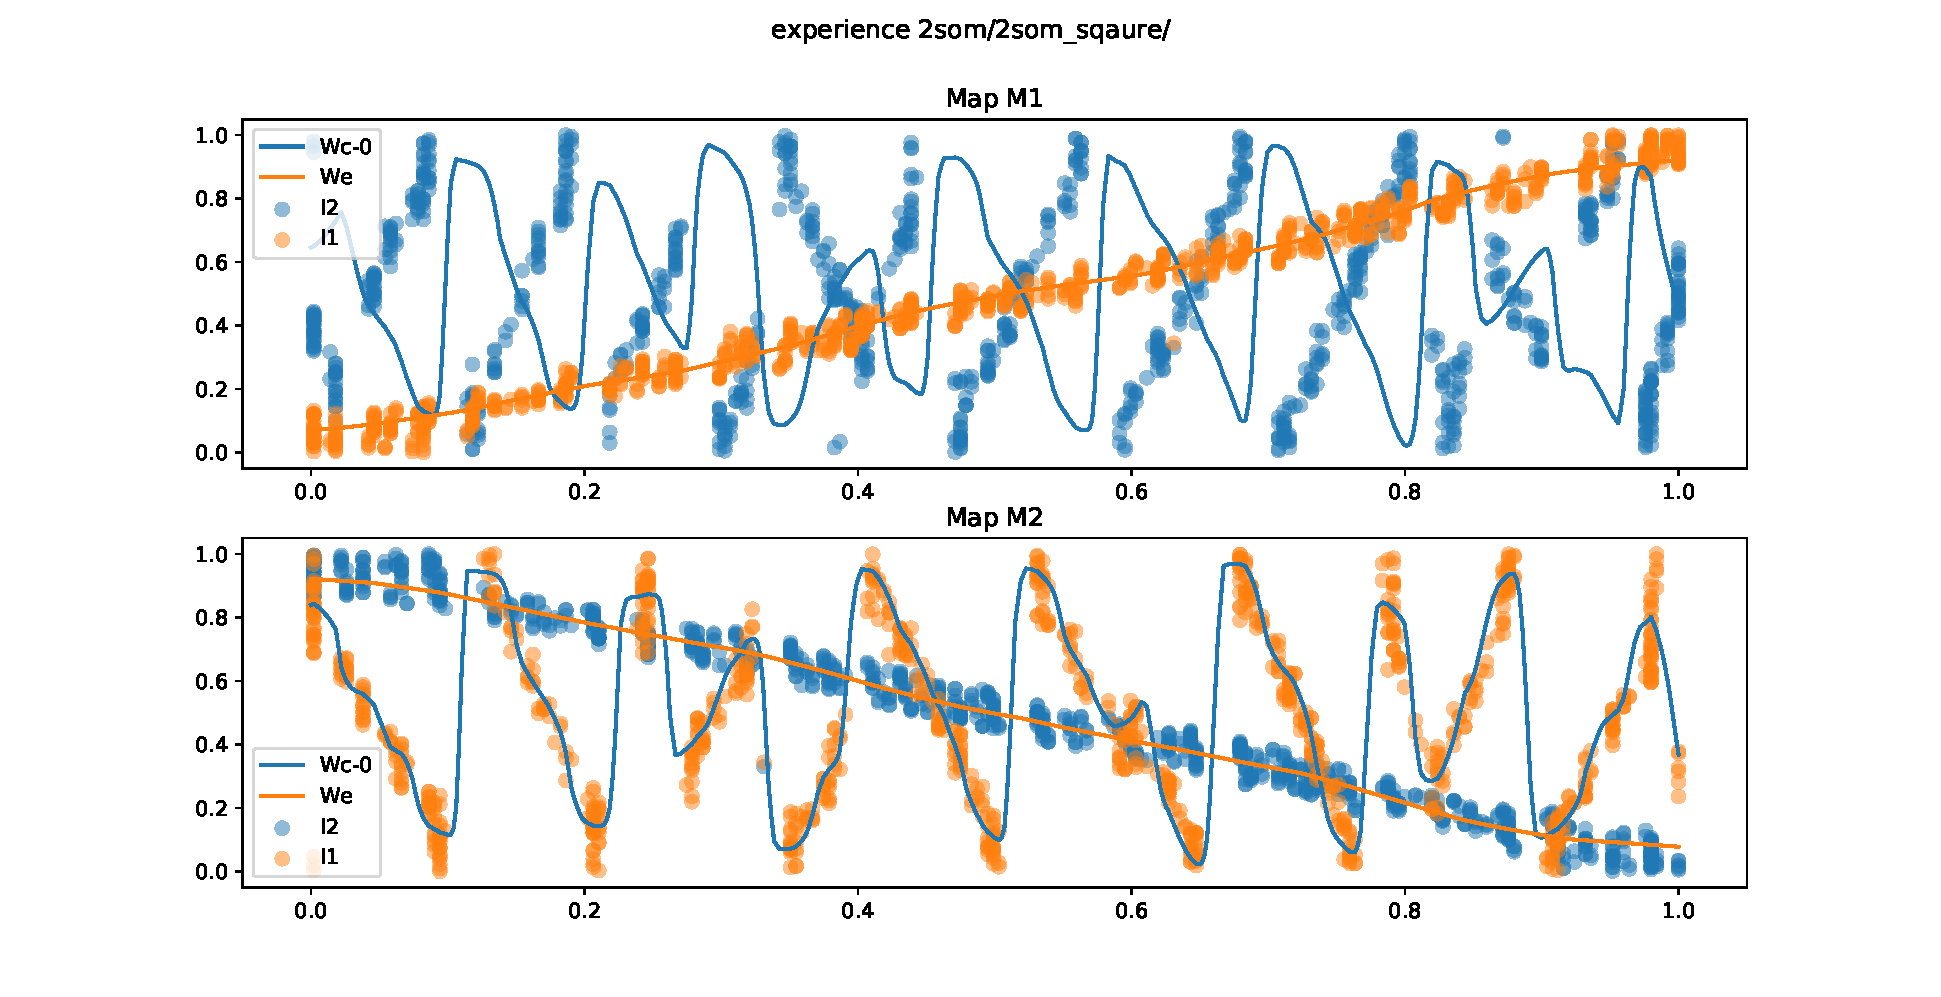
\includegraphics[width=\textwidth]{2som_square_w.pdf}
\end{minipage}
\begin{minipage}{0.33\textwidth}
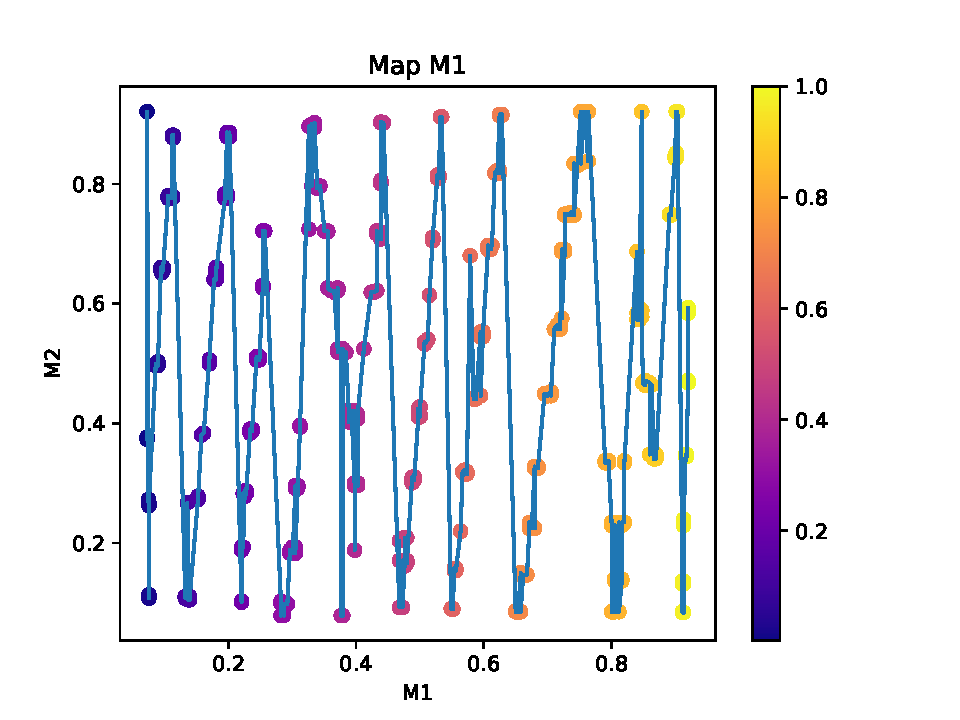
\includegraphics[width=\textwidth]{2som_square_d.pdf}
\end{minipage}
\begin{minipage}{0.33\textwidth}
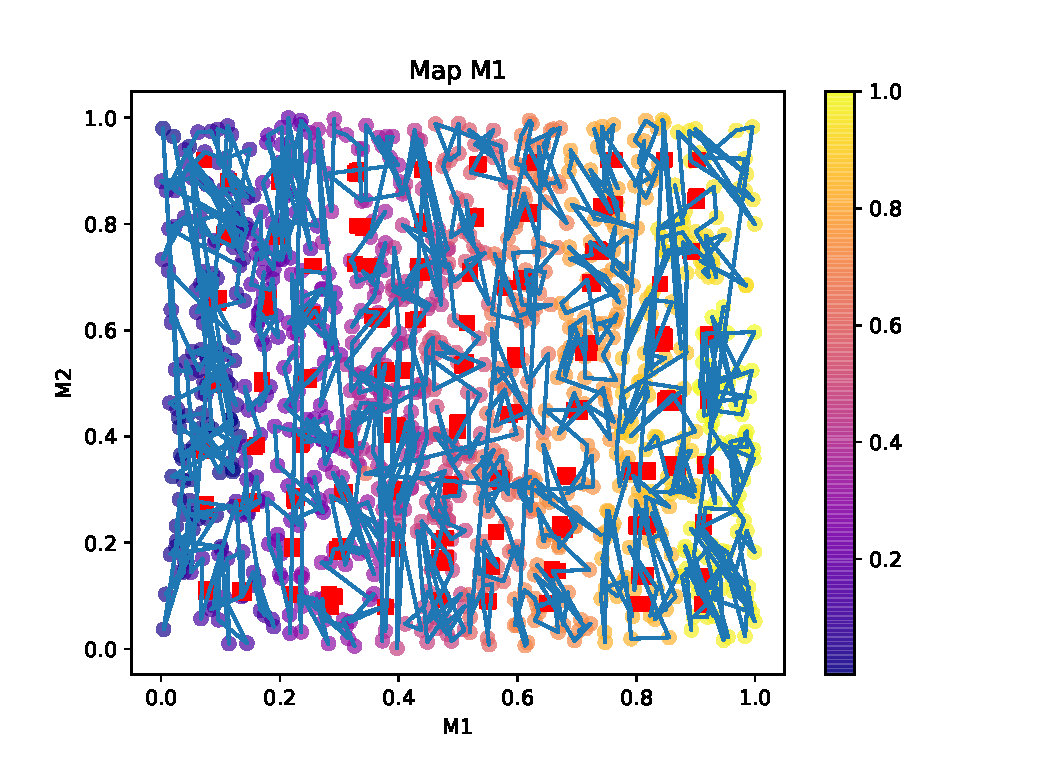
\includegraphics[width=\textwidth]{2som_square_din.pdf}
\end{minipage}
\label{fig:2som_square}
\caption{Tracé des poids de M1 et M2, dépliement des poids de M1 dans l'espace 2D et dépliement des entrées}
\end{figure}

Cette expérience montre que la disposition en vagues des cartes est un comportement lié à l'architecture et non aux données en elles même : quelles que soient les données, la carte effectuera toujours une séparation en indices primaires et secondaires. Ici, pour un X donné, on a toutes les valeurs possibles pour Y.
Cependant, les poids sont un peu différent de l'expérience avec X,Y sur un cercle : les bmus au sein d'une zone secondaire sont répartis tout le long de cette zone, alors que pour un cercle ils sont centrés dans la zone, car peu de valeurs possibles.